\chapter{Analiza wymagań}
Analiza wymagań jest kluczowym etapem procesu tworzenia oprogramowania. W jego trakcie dąży się do zrozumienie potrzeb użytkowników oraz przygotowanie poprawnej specyfikacji systemu. Analiza wymagań powinna uwzględniać także inne aspekty, związane np.\ ze skalowalnością, bezpieczeństwem i utrzymaniem systemu. W przypadku projektowania aplikacji typu eBOK dla wspólnoty mieszkaniowej, istotne jest zidentyfikowanie wszystkich funkcji wymaganych funkcji, które będą odpowiadały zarówno mieszkańcom, jak i administratorom, jak również przeanalizowanie kluczowych zagadnień dotyczących bezpieczeństwo, wydajności, intuicyjności interfejsu, architektury, a także integracji z innymi systemami. 

\section{Architektury systemu}
Zaprojektowanie architektury systemu jeszcze przed jego implementacją pozwala na stworzenie efektywnego i funkcjonalnego rozwiązania. Samo projektowanie architektury zwykle zaczyna się od naszkicowania jej zarysu, z wyszczególnieniem głównych komponentów systemu oraz ich wzajemnych interakcji. Taki szkic przedstawiono na rysunku~\ref{fig:zarys_architektury}. Widać na nim, że system składa się z kilku współpracujących ze sobą komponentów wdrożonych z wykorzystaniem konteneryzacji.
\begin{figure}[ht]
    \centering
    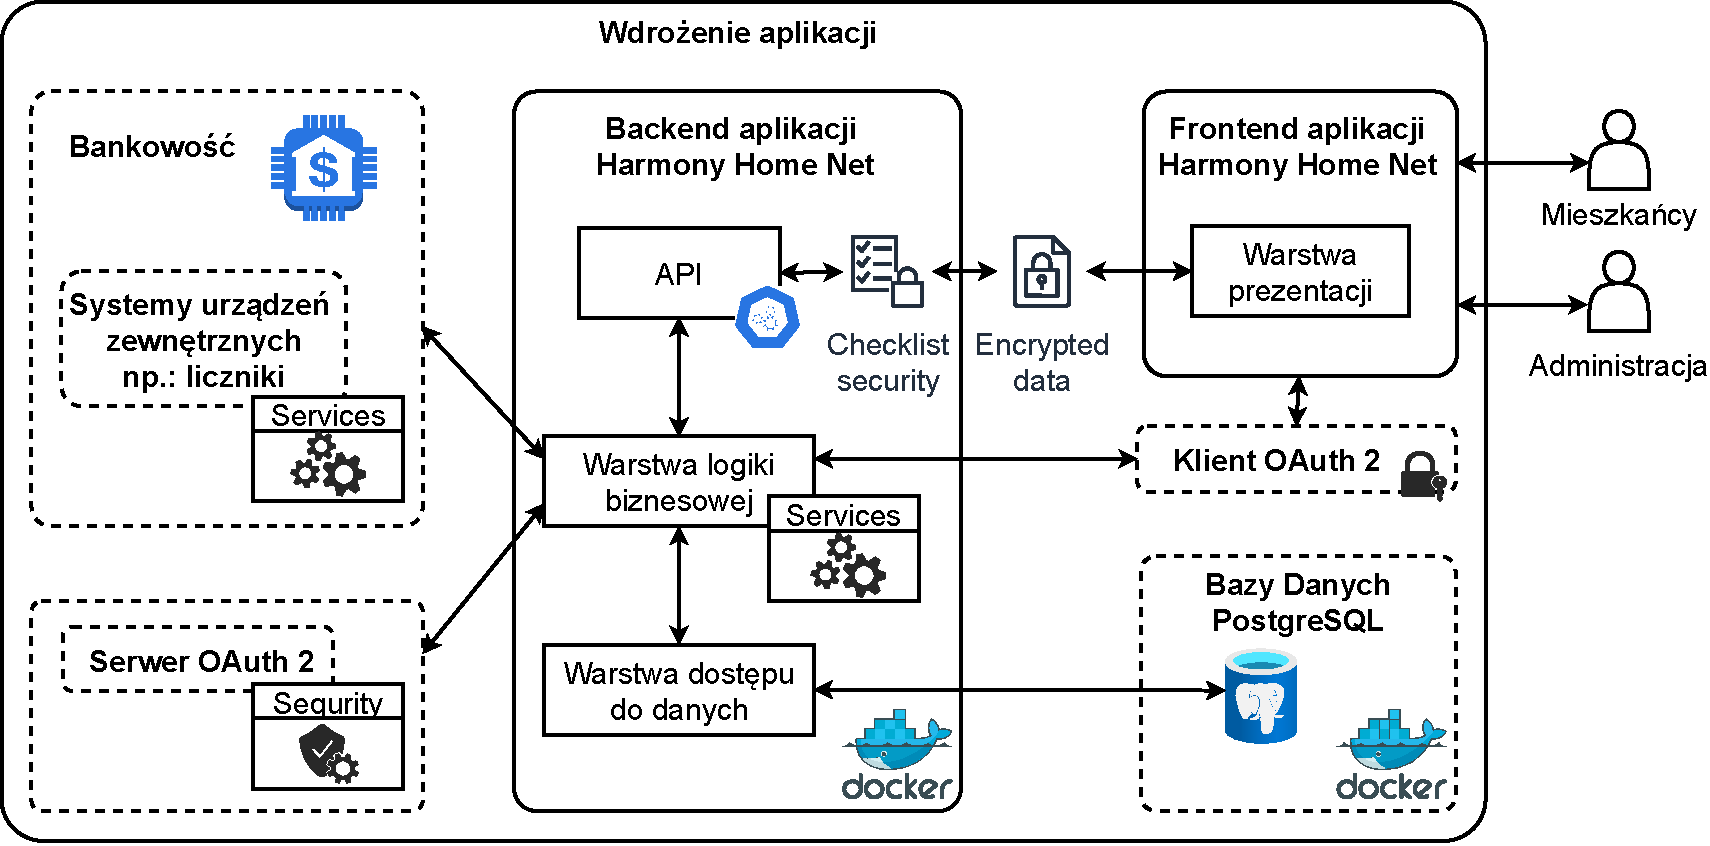
\includegraphics[width=\linewidth]{Schematy/zarys_architektury}
    \caption{Zarys architektury systemu „Harmony Home Net”}
    \label{fig:zarys_architektury}
\end{figure}


\subsection{Komponenty systemu}
System składać się ma z następujących komponentów: % TO DO: proszę doczytać (o co już prosiłem) zalecenia opisane w szablonie pracy (w szczególności Rozdział 5. Uwagi techniczne) i dostosować się do tych zaleceń.
\begin{itemize} 
	\item \textbf{Frontend} - Interfejs użytkownika aplikacji, zrealizowany w frameworku Next.js, pisany w TypeScript. Frontend obsługuje interakcje użytkowników (mieszkańców oraz administratorów) oraz prezentuje dane w odpowiednim formacie. Komunikacja z backendem odbywa się za pośrednictwem bezpiecznego protokołu HTTPS, a dane są szyfrowane przy pomocy protokołu TLS. Frontend (pokazany po prawej stronie na rys. \ref{fig:zarys_architektury}) pełni kluczową rolę w interakcji z użytkownikami, umożliwiając im dostęp do danych w łatwy sposób.

	\item \textbf{Backend} - Serwer aplikacji, oparty na Spring Boot, działający w kontenerze Docker, odpowiedzialny za logikę biznesową oraz zarządzanie danymi. Backend znajduje się centralnie na diagramie (rys. \ref{fig:zarys_architektury}) i odpowiada za funkcje takie jak autoryzacja użytkowników (przez OAuth 2.0), obsługa zgłoszeń mieszkańców, zarządzanie płatnościami i komunikacja z zewnętrznymi systemami. Konteneryzacja za pomocą Dockera (również widoczna na diagramie) zapewnia elastyczność i łatwość w skalowaniu.

	\item \textbf{Warstwa logiki biznesowej} - Kluczowa część backendu odpowiedzialna za implementację reguł biznesowych, która obsługują funkcje aplikacji, takie jak przetwarzanie zgłoszeń czy zarządzanie danymi użytkowników. Logika biznesowa, choć nie jest wyodrębniona na diagramie, stanowi centralną część backendu, odpowiadając za koordynację przepływu danych między frontendem, bazą danych oraz systemami zewnętrznymi.

	\item \textbf{Warstwa dostępu do danych} - Odpowiada za komunikację z bazą danych PostgreSQL, przechowującą informacje dotyczące użytkowników, zgłoszeń, płatności i innych istotnych danych. Ta warstwa zapewnia trwałość i integralność danych w systemie. W diagramie (rys. \ref{fig:zarys_architektury}), baza danych PostgreSQL jest zlokalizowana po prawej stronie, gdzie przechowuje wszystkie kluczowe informacje aplikacji.

	\item \textbf{Baza danych} - System wykorzystuje gotowy obraz Dockerowy PostgreSQL zamiast tworzenia nowej instancji bazy danych. Obraz ten zapewnia zarządzanie kluczowymi danymi aplikacji, takimi jak informacje o użytkownikach, zgłoszenia czy płatności. Dzięki zastosowaniu konteneryzacji, proces zarządzania bazą danych staje się prostszy i bardziej skalowalny ~\cite{Docker-docs,vsupalov}. Na diagramie (rys. \ref{fig:zarys_architektury}) baza danych PostgreSQL jest umieszczona po prawej stronie, gdzie współpracuje z backendem przy operacjach odczytu i zapisu danych.

	\item \textbf{Serwer OAuth 2.0} - Serwer autoryzacji, który zapewnia bezpieczeństwo dostępu do zasobów systemu przez użytkowników. OAuth 2.0 umożliwia zarządzanie autoryzacją dostępu, co zwiększa bezpieczeństwo aplikacji.

	\item \textbf{Systemy zewnętrzne} - Aplikacja integruje się z zewnętrznymi systemami, takimi jak bankowość (np. obsługa płatności online) oraz urządzenia zewnętrzne (np. liczniki zużycia mediów), co umożliwia kompleksową obsługę mieszkańców i automatyzację procesów. Zewnętrzne systemy znajdują się po lewej stronie diagramu, skąd integrują się z backendem w celu wymiany danych.


\end{itemize}

\subsection{Interakcje między komponentami}

Interakcje między komponentami są kluczowe dla sprawnego funkcjonowania systemu. W architekturze tej wykorzystano konteneryzację przy pomocy Dockera, co umożliwia izolowanie poszczególnych elementów systemu oraz ułatwia to skalowanie.

\begin{itemize} 
	\item \textbf{Frontend i Backend} - Frontend wysyła zapytania HTTPS do backendu (pokazanego pośrodku diagramu rys. \ref{fig:zarys_architektury}), poprzez zabezpieczenie protokołem TLS, w celu pobrania lub wysłania w sposób bezpieczny danych. Backend przetwarza te zapytania, wykonuje odpowiednie operacje na bazie danych i zwraca odpowiedzi do frontendu. Dane są wysyłane i odbierane w formacie JSON. Te interakcje są widoczne na schemacie jako przepływ między frontem po prawej a backendem w centrum.
	
	\item \textbf{Backend i Baza danych} - Backend łączy się z bazą danych PostgreSQL, która działa w kontenerze Docker, zapewniając niezależność środowiska oraz łatwość zarządzania i wdrażania. Gotowy obraz PostgreSQL usprawnia proces implementacji oraz dynamiczne skalowanie aplikacji, co ma kluczowe znaczenie dla jej wydajności i elastyczności~\cite{Docker-docs,vsupalov}.

	\item \textbf{Backend i System płatności} - Backend integruje się z systemami płatności, aby obsługiwać transakcje finansowe. Po dokonaniu płatności, system płatności przekazuje informacje zwrotne do backendu, który aktualizuje status płatności w bazie danych.

	\item \textbf{Backend i System powiadomień} - Backend wysyła powiadomienia do systemu powiadomień w celu informowania użytkowników o ważnych zdarzeniach. System powiadomień następnie dostarcza te informacje do użytkowników za pomocą e-maili lub SMS-ów.

\end{itemize}


\section{Wymagania aplikacji}

Aplikacja eBOK (Elektroniczne Biuro Obsługi Klienta) jest narzędziem wspierającym zarządzanie wspólnotami mieszkaniowymi, które ma na celu poprawę komunikacji pomiędzy mieszkańcami a administracją oraz automatyzację procesów związanych z obsługą nieruchomości. Jednym z kluczowych aspektów aplikacji jest zarządzanie lokalami, które w systemie pełnią centralną rolę, gdyż każda funkcja aplikacji – od zgłaszania usterek, przez płatności, po głosowania – jest związana z konkretnym lokalem.

Lokale, czyli nieruchomości (mieszkania, apartamenty, biura itp.), są podstawowym zasobem, który wymaga skutecznego zarządzania zarówno z perspektywy mieszkańca, jak i administratora. Dla mieszkańca lokal jest miejscem, do którego przypisane są należności finansowe, zgłoszenia techniczne czy dokumenty. Z perspektywy administratora, każdy lokal stanowi jednostkę, którą należy nadzorować pod kątem bieżących płatności, obsługi technicznej, jak również interakcji z właścicielami i najemcami. Dlatego zarządzanie lokalami/nieruchomościami w aplikacji eBOK jest jedną z kluczowych funkcji, zapewniającą przejrzystość oraz efektywność administracji.

\subsection{Przykłady użycia aplikacji}

Aplikacja eBOK oferuje różnorodne przypadki użycia, które ilustrują funkcje dostępne dla różnych grup użytkowników. Głównym obszarem jej zastosowania jest zarządzanie relacją pomiędzy mieszkańcem a administratorem nieruchomości, w kontekście takich działań jak płatności, zgłoszenia usterek, dostęp do dokumentów czy udział w głosowaniach. W aplikacji będzie można wyodrębnić 2 główne grupy użytkowników:

\begin{itemize} 

	\item \textbf{Mieszkańcy (właściciele i najemcy):} logując się do systemu, mają możliwość sprawdzenia należności za lokal, uregulowania opłat online oraz przeglądania historii rachunków. Mogą również zgłaszać usterki dotyczące lokalu (np. przeciek, awaria ogrzewania) i śledzić status zgłoszenia. Dodatkowo, mieszkaniecy ma dostęp do dokumentów związanych z jego lokalem, takich jak umowy, regulaminy czy faktury.
	
	\item \textbf{Administratorzy:} za pomocą panelu administracyjnego zarządzają zgłoszeniami technicznymi, przypisując je do wykonawców. Odpowiadają również za monitorowanie płatności związanych z każdym lokalem, a także za prowadzenie rejestru dokumentów i interakcje z mieszkańcami.
	
\end{itemize}

Każda z tych grup użytkowników ma dostęp do odpowiednich funkcji aplikacji, które spełniają jej potrzeby.

\subsection{Wymagania funkcjonalne}

Wymagania funkcjonalne aplikacji eBOK skupiają się na kluczowych obszarach działalności, które odpowiadają za sprawne funkcjonowanie wspólnoty mieszkaniowej.

\begin{enumerate}[label=\arabic*.]

	\item \textbf{Zarządzanie kontem użytkownika i lokalami:} Użytkownicy muszą mieć możliwość tworzenia kont, zarządzania swoimi danymi osobowymi oraz przypisywania lokali do konta. Mieszkańcy mogą być przypisani do wielu lokali, w zależności od tego, czy są właścicielami, czy najemcami. Funkcje dostępne dla mieszkańca są zależne od jego roli w danym lokalu (właściciel będzie miał znacząco większą ilość dostępnych funkcji w porównaniu do najemcy).

	\item \textbf{Przegląd i płatność należności:} Mieszkańcy mogą przeglądać szczegółowe informacje na temat należności przypisanych do konkretnego lokalu, którym zarządzają. Właściciele mają dostęp do pełnej historii opłat oraz możliwość ich realizacji online. Najemcy mogą jedynie przeglądać należności powiązane z ich umową najmu. System umożliwia szybki dostęp do historii opłat oraz realizację płatności online. Powiadomienia o zaległościach związanych z danym lokalem przypominają o konieczności uregulowania zobowiązań.

	\item \textbf{Zarządzanie zgłoszeniami technicznymi dla lokali:} Mieszkańcy (zarówno właściciele, jak i najemcy) mogą zgłaszać problemy techniczne dotyczące lokali, z którymi są powiązani. Właściciele mogą mieć dodatkowe uprawnienia do nadzorowania zgłoszeń związanych z większą liczbą lokali.

	\item \textbf{Zarządzanie dokumentami:} Lokale są również powiązane z dokumentami, takimi jak umowy najmu, protokoły przekazania, regulaminy czy faktury. Właściciele mają pełen dostęp do dokumentów powiązanych z ich lokalami, a najemcy mogą przeglądać dokumenty dotyczące tylko ich umowy najmu. Administratorzy zarządzają tymi dokumentami, przypisując je odpowiednim użytkownikom.

	\item \textbf{Głosowania mieszkańców:} W przypadku istotnych decyzji dotyczących zarządzania wspólnotą, administrator może organizować głosowania. Prawo głosu przysługuje mieszkańcom przypisanym do danego lokalu na podstawie ich roli (właściciel). Dzięki aplikacji proces głosowania jest zautomatyzowany, a wyniki są dostępne w czasie rzeczywistym.

	\item \textbf{Powiadomienia i komunikacja:} System powiadomień informuje użytkowników o ważnych wydarzeniach związanych z ich lokalem, takich jak zaległe płatności, zgłoszenia serwisowe czy nadchodzące głosowania. Rola użytkownika (właściciel lub najemca) determinuje, jakie powiadomienia są wysyłane oraz do których funkcji ma dostęp.

	\item \textbf{Panel administracyjny:} Administratorzy korzystają z zaawansowanego panelu, który pozwala im zarządzać wszystkimi lokalami, przypisywać mieszkańców do lokali, weryfikować uprawnienia użytkowników oraz monitorować zgłoszenia techniczne. Na podstawie umów lub dokumentów, administrator przypisuje lokale do nowych i istniejących kont mieszkańców.

	\item \textbf{Integracja z zewnętrznymi systemami:} Aplikacja eBOK musi umożliwiać integrację z systemami takimi jak systemy pomiarowe liczników mediów (np. wodomierze, liczniki energii) oraz systemy płatności. Taka integracja usprawnia zarządzanie lokalami, umożliwiając automatyczne generowanie rachunków oraz synchronizację danych dotyczących zużycia mediów.

	\item \textbf{Stany liczników:} System powinien umożliwiać użytkownikom wprowadzanie oraz przeglądanie stanów liczników powiązanych z danym lokalem, takich jak odczyty wodomierzy czy liczników energii. Aplikacja powinna automatycznie generować rozliczenia na podstawie wprowadzonych odczytów, co pozwala na dokładniejsze monitorowanie zużycia mediów oraz zarządzanie opłatami. Właściciele lokali mogą także mieć możliwość przeglądania historii odczytów i analizowania tendencji zużycia w czasie, co pomoże im lepiej planować wydatki i kontrolować koszty związane z mediami.
	
	\item \textbf{Forum mieszkańców:} System umożliwia utworzenie forum dyskusyjnego dla mieszkańców. Każdy mieszkaniec przypisany do lokalu, niezależnie od roli (właściciel, najemca), ma możliwość wzięcia udziału w dyskusjach, dodawania nowych tematów, odpowiadania na pytania innych mieszkańców oraz dzielenia się opiniami na temat zarządzania nieruchomościami, zgłoszeń technicznych czy innych spraw związanych ze wspólnotą. Administratorzy mogą moderować forum, usuwając nieodpowiednie treści oraz przypinając istotne informacje.


\end{enumerate}


\subsection{Wymagania niefunkcjonalne}

\begin{enumerate}[label=\arabic*.] 

	\item \textbf{Skalowalność:} System musi być na tyle elastyczny, aby mógł obsługiwać zarówno małe wspólnoty mieszkaniowe, jak i większe spółdzielnie, z możliwością zarządzania setkami lub tysiącami lokali aby obsłużyć rosnącą liczbę użytkowników oraz lokali bez znaczących spadków wydajności. Zastosowanie technologii Docker do konteneryzacji backendu i bazy danych PostgreSQL umożliwia łatwe skalowanie poziome (dodawanie kolejnych instancji), co pozwala na rozdzielenie obciążenia na większą liczbę serwerów.

	\item \textbf{Bezpieczeństwo:} Wszystkie dane użytkowników muszą być przechowywane i przesyłane w sposób bezpieczny. Wymagane jest szyfrowanie komunikacji między frontendem a backendem (TLS), a także autoryzacja użytkowników za pomocą OAuth 2.0. Ponadto system musi chronić dane przed nieautoryzowanym dostępem, co obejmuje zabezpieczenia na poziomie aplikacji, takie jak ograniczenie dostępu do funkcji na podstawie roli użytkownika (np. właściciel, najemca, administrator), uwierzytelnianie dwuskładnikowe oraz ochronę przed zagrożeniami takimi jak ataki SQL Injection czy XSS.

	\item \textbf{Wydajność:} System powinien być responsywny, zapewniając jak najszybszy możliwy czas odpowiedzi na zapytanie. Backend oparty na Spring Boot oraz baza danych PostgreSQL muszą być odpowiednio zoptymalizowane pod kątem operacji zapisu i odczytu, aby sprostać wymaganiom w czasie rzeczywistym, szczególnie podczas obciążeń związanych z masowym przetwarzaniem danych (np. zgłoszenia techniczne, płatności).

	\item \textbf{Dostępność:} Aplikacja powinna być dostępna przez 99,9\% czasu, z minimalnymi przerwami na konserwację. Wdrożenie technologii kontenerowej (Docker) oraz monitorowanie serwerów w czasie rzeczywistym pozwala na szybkie identyfikowanie problemów i automatyczne odzyskiwanie usług w przypadku awarii.

	\item \textbf{Intuicyjność interfejsu:} Aplikacja musi być łatwa w obsłudze zarówno dla mieszkańców, jak i administratorów. Intuicyjny interfejs, oparty na komponentach Shadcn UI i zgodny z wytycznymi WCAG 2.0, zapewnia łatwy dostęp do funkcji. Ocenę intuicyjności można przeprowadzić na podstawie testów akceptacyjnych, w których użytkownicy będą oceniali łatwość korzystania z systemu.
	
	\item \textbf{Zgodność z przepisami RODO:} System musi spełniać wymagania dotyczące ochrony danych osobowych, wynikające z RODO. Oznacza to, że wszystkie dane osobowe przechowywane w systemie muszą być chronione, użytkownicy muszą mieć możliwość wglądu w swoje dane, ich modyfikacji, a także żądania ich usunięcia. Przetwarzanie danych osobowych musi być odpowiednio udokumentowane, a dostęp do tych danych powinien być ograniczony.

	\item \textbf{Niezawodność:} System musi zapewniać ciągłość działania oraz zachowywać dane użytkowników nawet w przypadku awarii serwera. Konieczne jest wdrożenie mechanizmów regularnych kopii zapasowych bazy danych oraz planu odzyskiwania po awarii, który umożliwia szybkie przywrócenie systemu do pełnej funkcjonalności w krótkim czasie.

	\item \textbf{Testowalność:} Każda z funkcji aplikacji powinna być możliwa do przetestowania w sposób automatyczny, co umożliwi szybkie wykrywanie błędów w kodzie. Testy automatyczne powinny obejmować testy jednostkowe, integracyjne oraz systemowe, sprawdzając poprawność działania każdej funkcji zarówno z poziomu frontendu, jak i backendu. Testy akceptacyjne powinny obejmować scenariusze użytkownika, weryfikując, czy system spełnia wymagania stawiane przez administratorów i mieszkańców.

	\item \textbf{Elastyczność:} System powinien umożliwiać łatwe wprowadzanie nowych funkcji lub modyfikację istniejących bez konieczności przeprowadzania szerokich zmian w kodzie. Architektura warstwowa (N-tier), z wyraźnym rozdzieleniem logiki biznesowej, danych oraz interfejsu użytkownika, zapewnia elastyczność oraz ułatwia przyszły rozwój aplikacji.
	
\end{enumerate}

\section{Podsumowanie}

Analiza wymagań dla systemu „Harmony Home Net” jest kluczowym krokiem w kierunku zaprojektowania i implementacji aplikacji, która sprosta potrzebom zarówno mieszkańców, jak i administratorów wspólnot mieszkaniowych. Wymagania funkcjonalne i niefunkcjonalne omówione w tym rozdziale stanowią podstawę do dalszego projektowania systemu oraz planowania jego architektury. Umożliwiają one stworzenie aplikacji, która będzie nie tylko spełniać oczekiwania użytkowników, ale także zapewniać wysoki poziom bezpieczeństwa, wydajności i skalowalności, niezbędnych do efektywnego zarządzania nieruchomościami.
